%%%%%%%%%%%%%%%%%%%%%%%%%%%%%%%%%%%%%%%%%
% Short Sectioned Assignment LaTeX Template Version 1.0 (5/5/12)
% This template has been downloaded from: http://www.LaTeXTemplates.com
% Original author:  Frits Wenneker (http://www.howtotex.com)
% License: CC BY-NC-SA 3.0 (http://creativecommons.org/licenses/by-nc-sa/3.0/)
%%%%%%%%%%%%%%%%%%%%%%%%%%%%%%%%%%%%%%%%%

%----------------------------------------------------------------------------------------
%	PACKAGES AND OTHER DOCUMENT CONFIGURATIONS
%----------------------------------------------------------------------------------------

\documentclass[paper=a4, fontsize=11pt]{scrartcl} % A4 paper and 11pt font size

% ---- Entrada y salida de texto -----

\usepackage[T1]{fontenc} % Use 8-bit encoding that has 256 glyphs
\usepackage[utf8]{inputenc}
%\usepackage{fourier} % Use the Adobe Utopia font for the document - comment this line to return to the LaTeX default

% ---- Idioma --------

\usepackage[spanish, es-tabla]{babel} % Selecciona el español para palabras introducidas automáticamente, p.ej. "septiembre" en la fecha y especifica que se use la palabra Tabla en vez de Cuadro

% ---- Otros paquetes ----

\usepackage{url} % ,href} %para incluir URLs e hipervínculos dentro del texto (aunque hay que instalar href)
\usepackage{amsmath,amsfonts,amsthm} % Math packages
%\usepackage{graphics,graphicx, floatrow} %para incluir imágenes y notas en las imágenes
\usepackage{graphics,graphicx, float} %para incluir imágenes y colocarlas

% Para hacer tablas comlejas
%\usepackage{multirow}
%\usepackage{threeparttable}

%\usepackage{sectsty} % Allows customizing section commands
%\allsectionsfont{\centering \normalfont\scshape} % Make all sections centered, the default font and small caps

\usepackage{fancyhdr} % Custom headers and footers
\pagestyle{fancyplain} % Makes all pages in the document conform to the custom headers and footers
\fancyhead{} % No page header - if you want one, create it in the same way as the footers below
\fancyfoot[L]{} % Empty left footer
\fancyfoot[C]{} % Empty center footer
\fancyfoot[R]{\thepage} % Page numbering for right footer
\renewcommand{\headrulewidth}{0pt} % Remove header underlines
\renewcommand{\footrulewidth}{0pt} % Remove footer underlines
\setlength{\headheight}{13.6pt} % Customize the height of the header

\numberwithin{equation}{section} % Number equations within sections (i.e. 1.1, 1.2, 2.1, 2.2 instead of 1, 2, 3, 4)
\numberwithin{figure}{section} % Number figures within sections (i.e. 1.1, 1.2, 2.1, 2.2 instead of 1, 2, 3, 4)
\numberwithin{table}{section} % Number tables within sections (i.e. 1.1, 1.2, 2.1, 2.2 instead of 1, 2, 3, 4)

\setlength\parindent{0pt} % Removes all indentation from paragraphs - comment this line for an assignment with lots of text

\newcommand{\horrule}[1]{\rule{\linewidth}{#1}} % Create horizontal rule command with 1 argument of height

\graphicspath{ {./images/} }
\usepackage{subcaption}
\usepackage{hyperref}
\usepackage{soul}

%----------------------------------------------------------------------------------------
%	TÍTULO Y DATOS DEL ALUMNO
%----------------------------------------------------------------------------------------

\title{	
\normalfont \normalsize 
\textsc{\textbf{Aprendizaje Automático (2019)} \\ Doble Grado en Ingeniería Informática y Matemáticas \\ Universidad de Granada} \\ [25pt] % Your university, school and/or department name(s)
\horrule{0.5pt} \\[0.4cm] % Thin top horizontal rule
\huge Memoria Práctica 1 \\ % The assignment title
\horrule{2pt} \\[0.5cm] % Thick bottom horizontal rule
}

\author{Luis Balderas Ruiz \\ \texttt{luisbalderas@correo.ugr.es}} 
 % Nombre y apellidos 


\date{\normalsize\today} % Incluye la fecha actual

%----------------------------------------------------------------------------------------
% DOCUMENTO
%----------------------------------------------------------------------------------------

\begin{document}

\maketitle % Muestra el Título

\newpage %inserta un salto de página

\tableofcontents % para generar el índice de contenidos

\listoffigures

\listoftables

\newpage


%----------------------------------------------------------------------------------------
%	Introducción
%----------------------------------------------------------------------------------------

\section{EJERCICIO SOBRE LA BÚSQUEDA ITERATIVA DE ÓPTIMOS}

\subsection{Gradiente Descendente}

\subsubsection{Implementación del algoritmo de gradiente descendente}

Gradiente descendente es un algoritmo muy general que puede ser usado para entrenar una gran cantidad de modelos de aprendizaje consiguiendo errores pequeños. Desde un punto de vista más matemático, es una ténica que busca minimizar funciones dos veces derivables. \cite{lfd}. Más concretamente, gradiente descendente trabaja en espacios de cualquier dimensión, incluso de dimensión infinita. En este caso, el espacio de búsqueda es un espacio de funciones donde se calcula la derivada de Fréchet del funcional a minimizar para determinar la dirección descendente \cite{funtional_analysis}. \\

En el marco de nuestro desarrollo teórico, gradiente descendente se ha presentado como una técnica de estimación paramétrica, en la que, dado un conjunto de entrenamiento y sus correspondientes, se pretende minimizar el error cometidos en las predicciones de las etiquetas sobre dichos puntos (lo que venimos llamando $E_{in}$) de cara a adquirir un conocimiento extrapolable a tuplas no examinadas (el conjunto de test). Sin embargo, en esta práctica se pretende enfocar este algoritmo como una herramienta de minimización de funciones. Por tanto, es necesario variar el esquema definido en clase y establecer un criterio de parada acorde a nuestro objetivo, esto es, minimizar una función. Teniéndolo en cuenta, tomo como criterio de parada el hecho de que la diferencia entre la imagen de dos puntos consecutivos predichos sea más pequeña que una tolerancia. En otras palabras, si $f$ es la función que queremos minimizar y $w_1,w_2$ son valores consecutivos,

$$\text{Dado un } \epsilon > 0, \text{ si } |f(w_1)-f(w_2)| < \epsilon \Rightarrow \text{ PARADA }$$


He de añadir que mi algoritmo devuelve el valor mínimo encontrado ($w$), el número de iteraciones necesarias para encontrarlo y una lista con las distintas imágenes de la función para así ver como va disminuyendo.

\subsubsection{Función $E(u,v) = (u^2e^v-2v^2e^{-u})^2$}

Considero la función $E(u,v) = (u^2e^v-2v^2e^{-u})^2$. Como se puede ver, es una función de clase $C^{\infty}$ respecto de las dos variables, luego es factible utilizar el gradiente descendente para encontrar su mínimo. Tomando $\eta=0.01$ y empezando en $(u,v)=(1,1)$, calculo el mínimo. \\

Primero, calculo el gradiente de la función $E(u,v)$:
$$\frac{\partial E(u,v)}{\partial u} = (u^2e^v-2v^2e^{-u})(4ue^v+4v^2e^{-v})$$
$$\frac{\partial E(u,v)}{\partial v} = (2u^2e^v-8ve^{-u})(u^2e^v-2v^2e^{-u})$$

$$\Rightarrow \nabla E(u,v) = \left((4ue^v+4v^2e^{-v})(u^2e^v-2v^2e^{-u}),(u^2e^v-2v^2e^{-u})(2u^2e^v-8ve^{-u})\right)$$

Dado $\epsilon = 10^{-14}$, el número de iteraciones necesarias para obtener un valor por debajo de esa tolerancia (usando flotantes de 64 bits) es 34. Dicho valor se da en el par $(x,y) = (0.619207671834479,0.968448270676094)$

Podemos observarlo en la siguiente gráfica, en la que vemos como converge muy rápidamente (basta una iteración para que se acerque mucho al punto final) hasta que en el 34 se da el criterio de parada. \\

\begin{figure}[H] %con el [H] le obligamos a situar aquí la figura
	\centering
	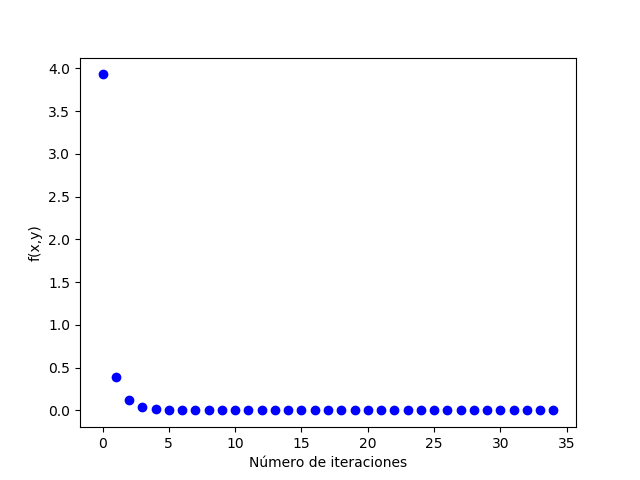
\includegraphics[scale=0.6]{e1.png}  %el parámetro scale permite agrandar o achicar la imagen. En el nombre de archivo puede especificar directorios
	\caption{Progresión de la imagen de E en cada iteración} 
	\label{fig:e1}
\end{figure}

\subsubsection{Función $f(x,y)=x^2+2y^2+2sin(2\pi x) sin(2\pi y)$}

En este caso trabajo con la función $f(x,y)=x^2+2y^2+2sin(2\pi x) sin(2\pi y)$. Esta función vuelve a ser clase $C^{\infty}$, luego podemos aplicar gradiente descendente sin problema. Tomando como punto inicial $(x_0,y_0) = (0.1,0.1), \eta = 0.01$ y un máximo de 50 iteraciones, minimizo la función y muestro el gráfico correspondiente. Como se puede ver, la convergencia se produce cerca de la duodécima iteración para llegar a la parada en la número 24. Las coordenadas del mínimo obtenido son $(x,y) = (0.24380496934646,-0.237925821480742$)

\begin{figure}[H] %con el [H] le obligamos a situar aquí la figura
	\centering
	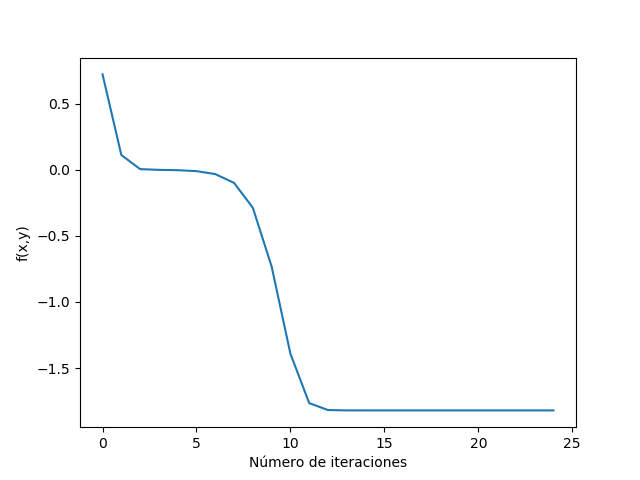
\includegraphics[scale=0.6]{f1.png}  %el parámetro scale permite agrandar o achicar la imagen. En el nombre de archivo puede especificar directorios
	\caption{Progresión de la imagen de f en cada iteración} 
	\label{fig:f1}
\end{figure}

Si dibujamos el contorno de esta función, podemos ver que existen varias zonas con mínimos y que, empezando en el par indicado antes, por la proximidad que presenta, cae en el mínimo obtenido.

\begin{figure}[H] %con el [H] le obligamos a situar aquí la figura
	\centering
	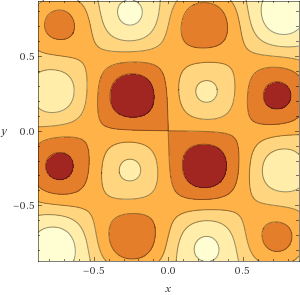
\includegraphics[scale=0.6]{f2.png}  %el parámetro scale permite agrandar o achicar la imagen. En el nombre de archivo puede especificar directorios
	\caption{El mínimo alcanzado es cercano al punto inicial, luego la convergencia es lógica} 
	\label{fig:f2}
\end{figure}


Para el caso en el que $\eta=0.1$ vamos a observar que no hay una convergencia, ya que, al ser un learning rate alto, se producen saltos que imposibilitan el descenso al mínimo. Así lo muestra la siguiente gráfica:

\begin{figure}[H] %con el [H] le obligamos a situar aquí la figura
	\centering
	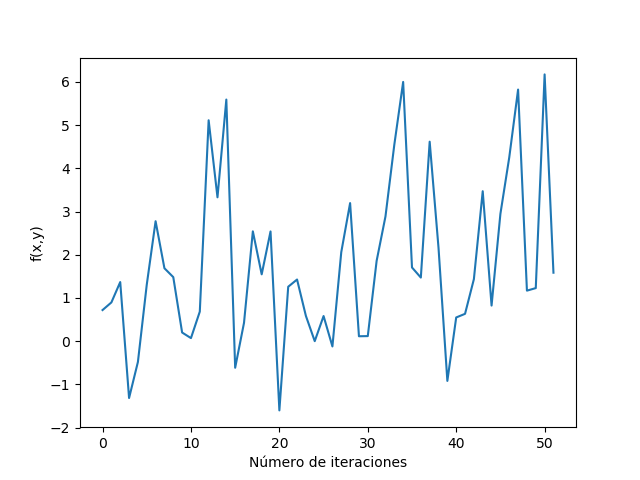
\includegraphics[scale=0.6]{f3.png}  %el parámetro scale permite agrandar o achicar la imagen. En el nombre de archivo puede especificar directorios
	\caption{Nube de puntos consecuencia del learning rate = 0.1} 
	\label{fig:f3}
\end{figure}

Por tanto, vemos que ajustar el valor del learning rate es determinante para conseguir buenos resultados. Con esta idea, en el siguiente ejercicio, en el que no se ponen restricciones sobre los parámetros, desarrollo un pequeño estudio sobre el conjunto de valores apropiado que puede tomar la tasa de aprendizaje. Por otra parte, una tasa de aprendizaje constante acaba por tener un peor rendimiento en el proceso de minimización, ya que, para un $w$ cercano al mínimo, $\eta$ debería ir disminuyendo. De esta forma conseguiríamos una convergencia mucho más rápida. En ese sentido, se presenta el Gradiente Descendente Rápido (Faster Gradient Descent), a través de un learning rate adaptativo \cite{fgd}.

\subsubsection{Evaluación en distintos puntos}

Probamos ahora el algoritmo en distintos puntos iniciales para ver la importancia de este parámetro de entrada y para constatar, una vez más, que gradiente descendente es un algoritmo que garantiza encontrar mínimos locales (la derivada es un concepto local). En la primera columna de la tabla se encuentran los puntos iniciales, a continuación, los mínimos encontrados y, finalmente, la imagen de estos.

\begin{table}[H]
	\begin{tabular}{|c|c|c|}
		\hline
		$(x_0,y_0)$   & $(x,y)$ (Valor donde se alcanza el mínimo)                                 & $f(x,y)$          \\ \hline
		$(0.1,0.1)$   & $(0.243804969346460, -0.237925821480742)$  & -1.82007854154716 \\ \hline
		$(1,1)$       & $(1.21807030090520, 0.712811950338754)$    & 0.593269374325836 \\ \hline
		$(-0.5,-0.5)$ & $(-0.731377459870107, -0.237855362955527)$ & -1.33248106233098 \\ \hline
		$(-1,-1)$     & $(-1.21807030090520, -0.712811950338754)$  & 0.593269374325836 \\ \hline
	\end{tabular}
	\caption{Tabla requerida en el ejercicio 3 b)}
	\label{table1}
\end{table}

\subsubsection{Conclusión sobre la verdadera dificultad de encontrar el mínimo global de una función arbitraria}




\newpage
\section{Bibliografía}

%------------------------------------------------

\bibliography{citas} %archivo citas.bib que contiene las entradas 
\bibliographystyle{plain} % hay varias formas de citar

\end{document}
